\documentclass{article}
\usepackage{pgfplots}
\pgfplotsset{width=9cm,compat=1.5}
\begin{document}

%Ram time
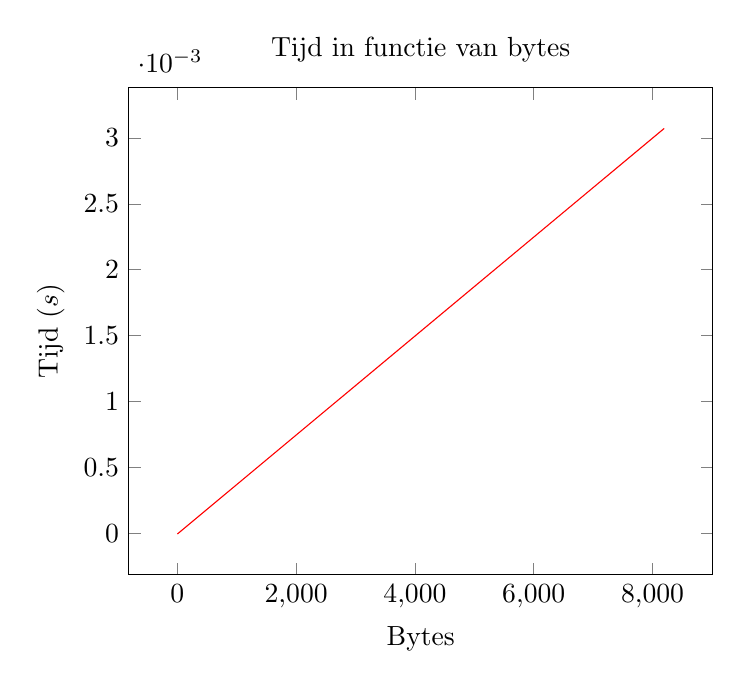
\begin{tikzpicture}
\begin{axis}[
title=Tijd in functie van bytes,
xlabel={Bytes},
ylabel={Tijd $(s)$}
]
\addplot[
red,
domain=0:8196,
samples=201,
]
{3.752E-7 *x -3.773E-6};
\end{axis}
\end{tikzpicture}

%Ram energy
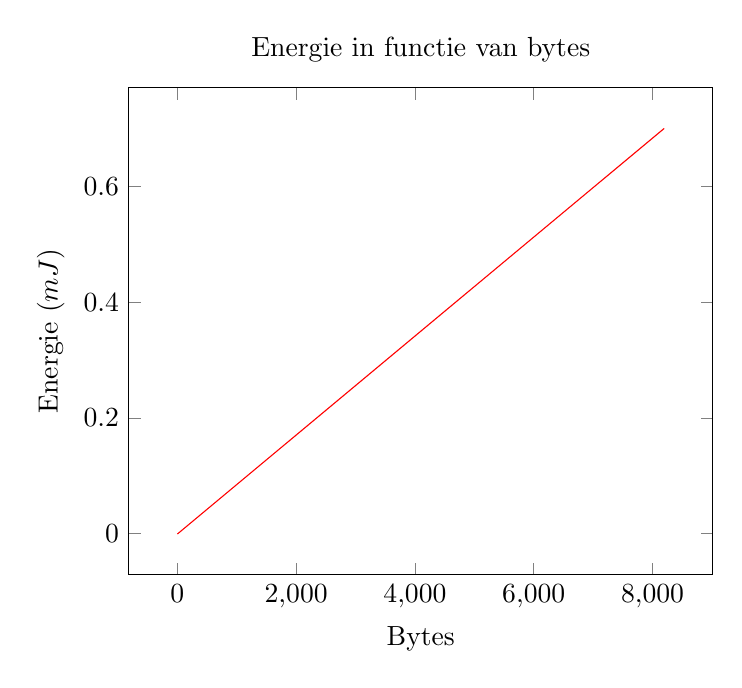
\begin{tikzpicture}
\begin{axis}[
title=Energie in functie van bytes,
xlabel={Bytes},
ylabel={Energie $(mJ)$}
]
\addplot[
red,
domain=0:8196,
samples=201,
]
{8.559E-5 * x - 1.019E-3};
\end{axis}
\end{tikzpicture}

%CPU engergie
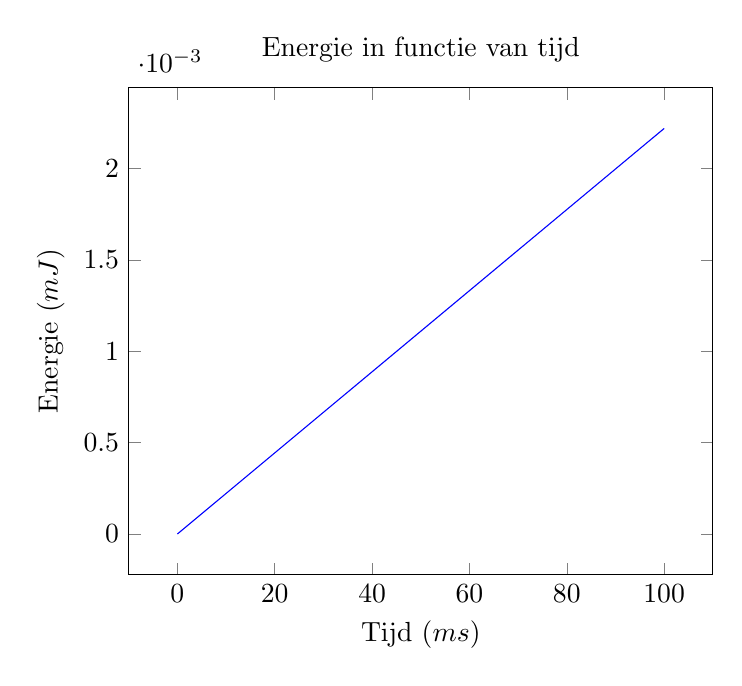
\begin{tikzpicture}
\begin{axis}[
title=Energie in functie van tijd,
xlabel={Tijd $(ms)$},
ylabel={Energie $(mJ)$}
]
\addplot[
blue,
domain=0:100,
samples=201,
]
{0.0037 * x *1E-3 *6};
\end{axis}
\end{tikzpicture}

%Antenne energie
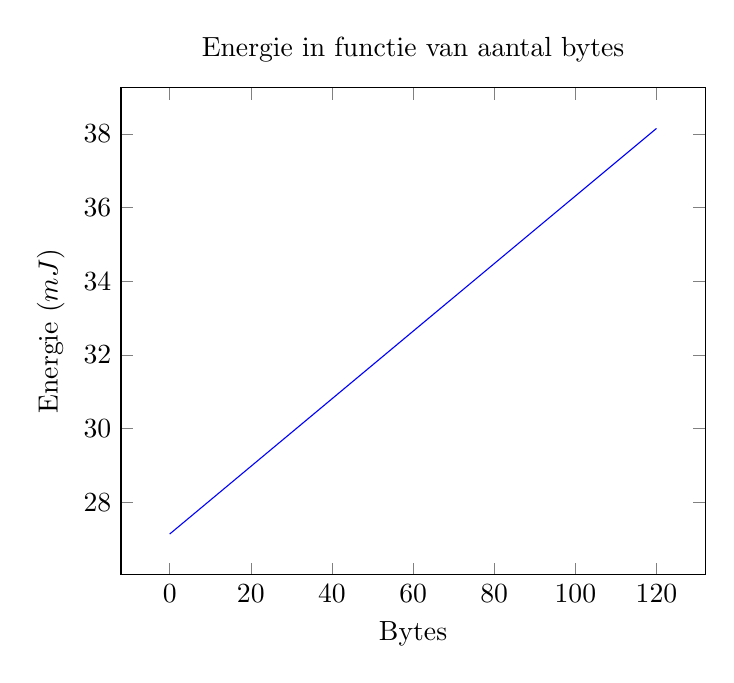
\begin{tikzpicture}
\begin{axis}[
title=Energie in functie van aantal bytes,
xlabel={Bytes},
ylabel={Energie $(mJ)$}
]
\addplot[
blue,
domain=0:120,
samples=201,
]
{0.04 * (x * 0.382 + 113.104)*6};
\end{axis}
\end{tikzpicture}
\end{document}